\chapter{Analyse fonctionnel}

Compte tenu des recherches que nous avons réalisées, nous avons établi l'étude fonctionnelle suivante.

\section{Diagramme pieuvre}

\hspace{-2cm}
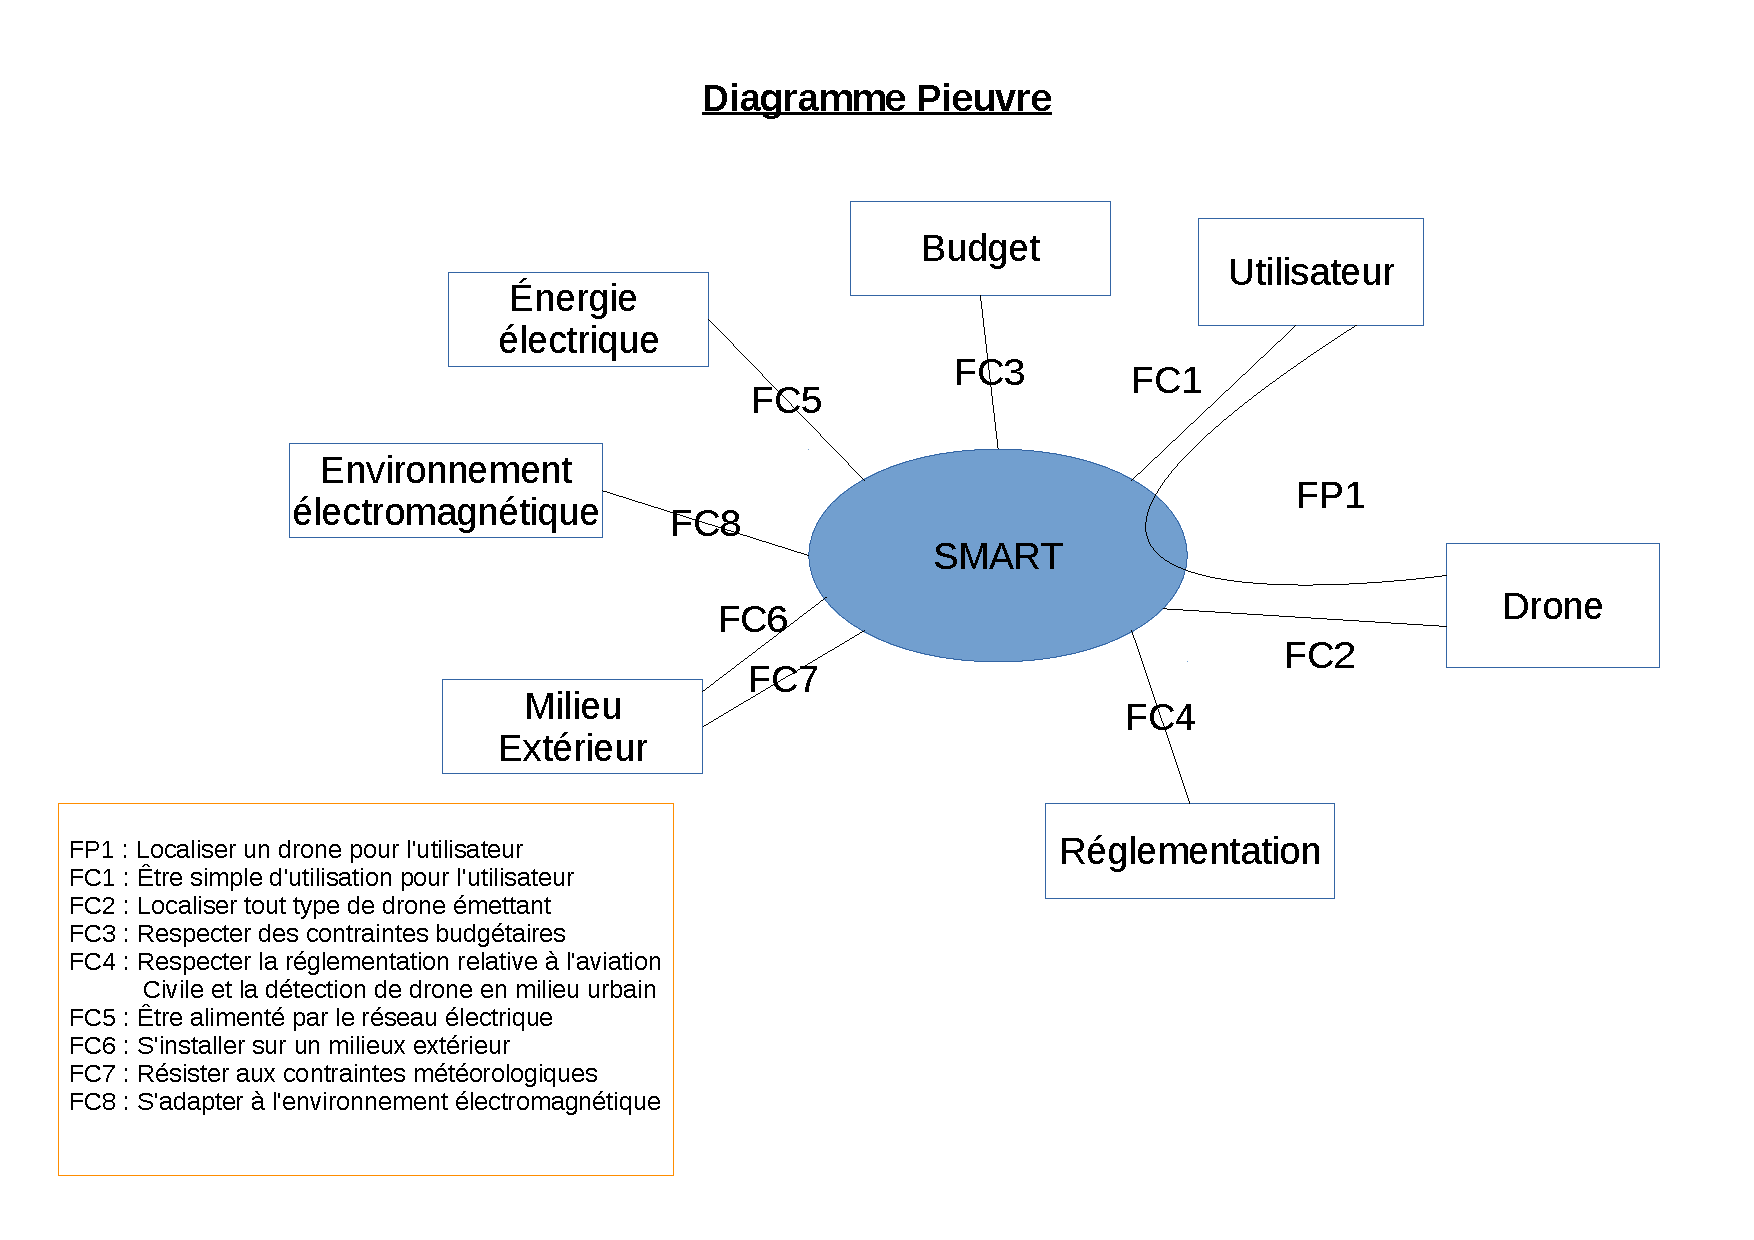
\includegraphics[width=1.18\textwidth]{Diagramme_pieuvre.pdf}
\captionof{figure}{Diagramme pieuvre}



\section{SADT}

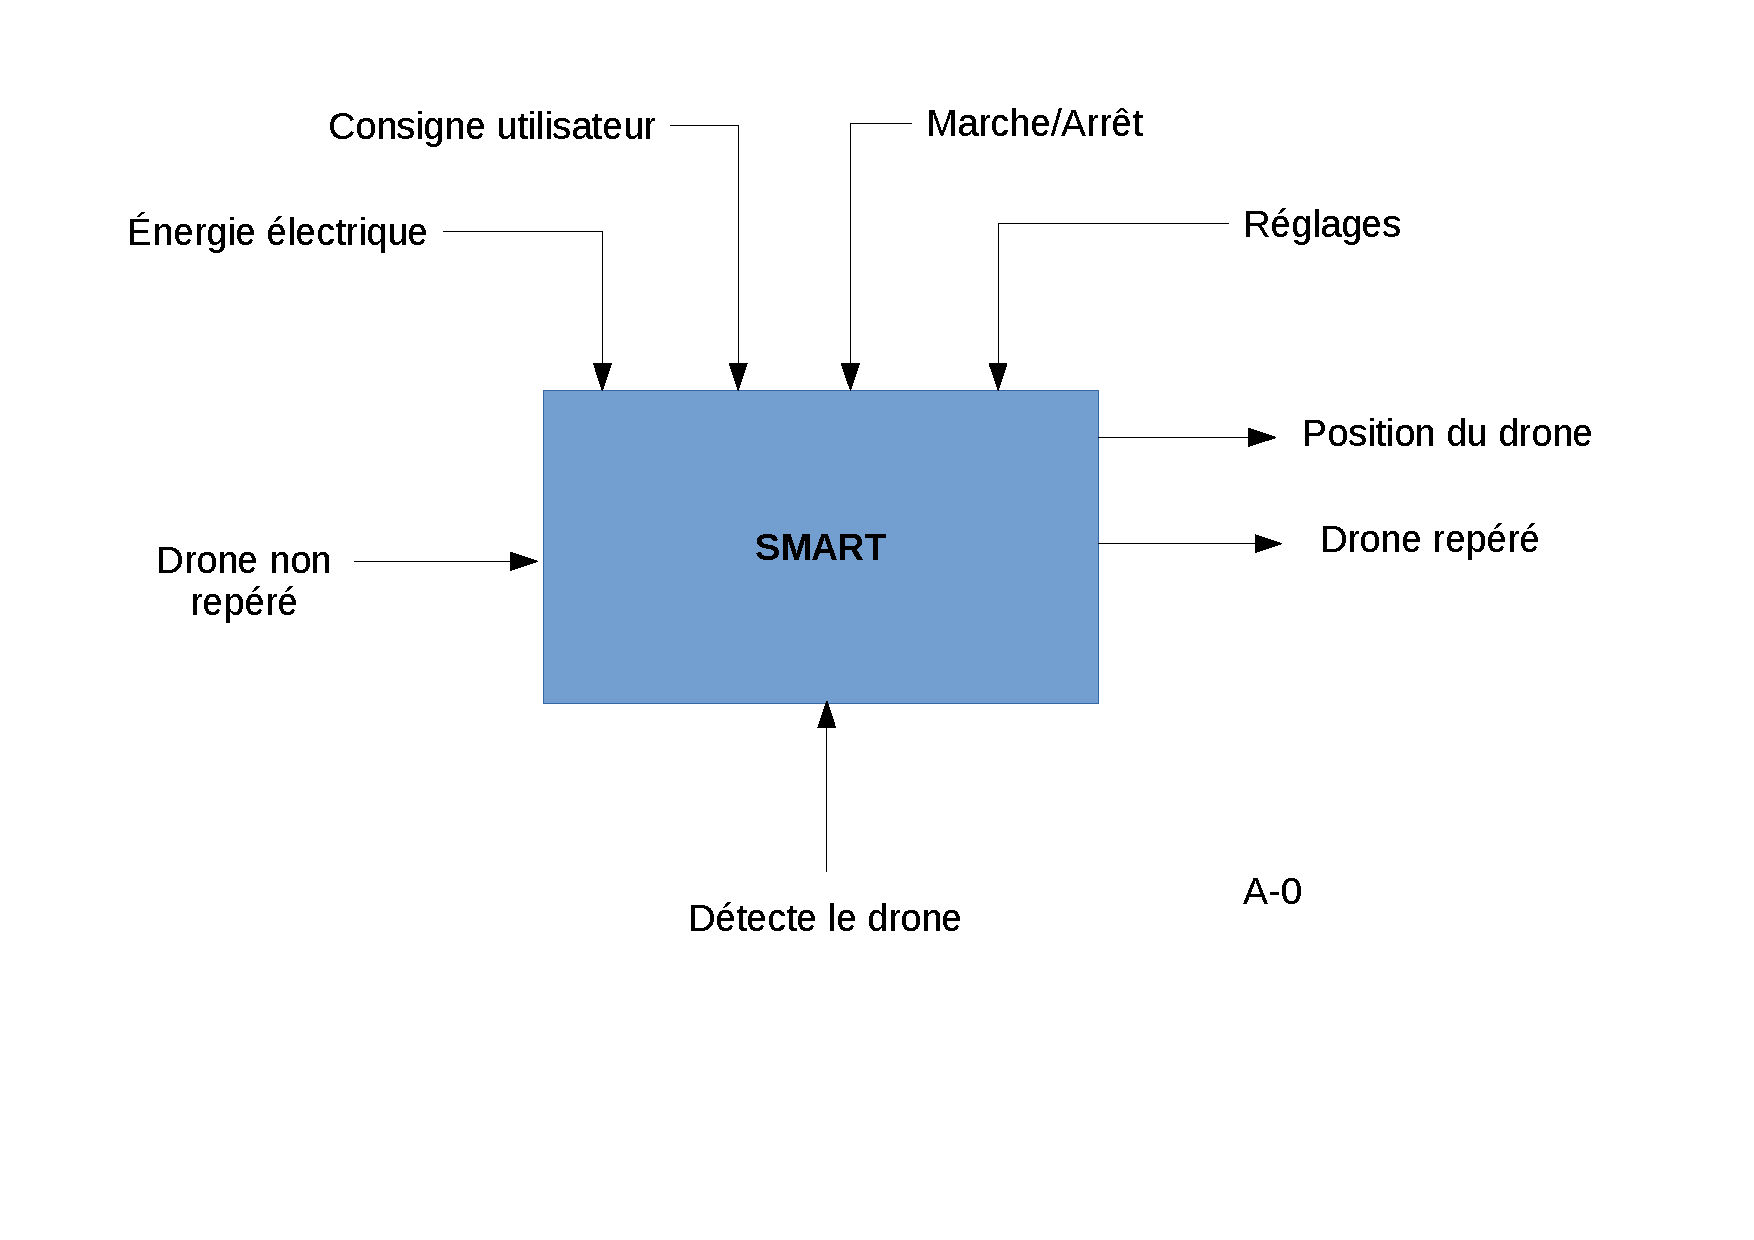
\includegraphics[width=\textwidth]{SADT_A-0.pdf}
\captionof{figure}{SADT A-0}
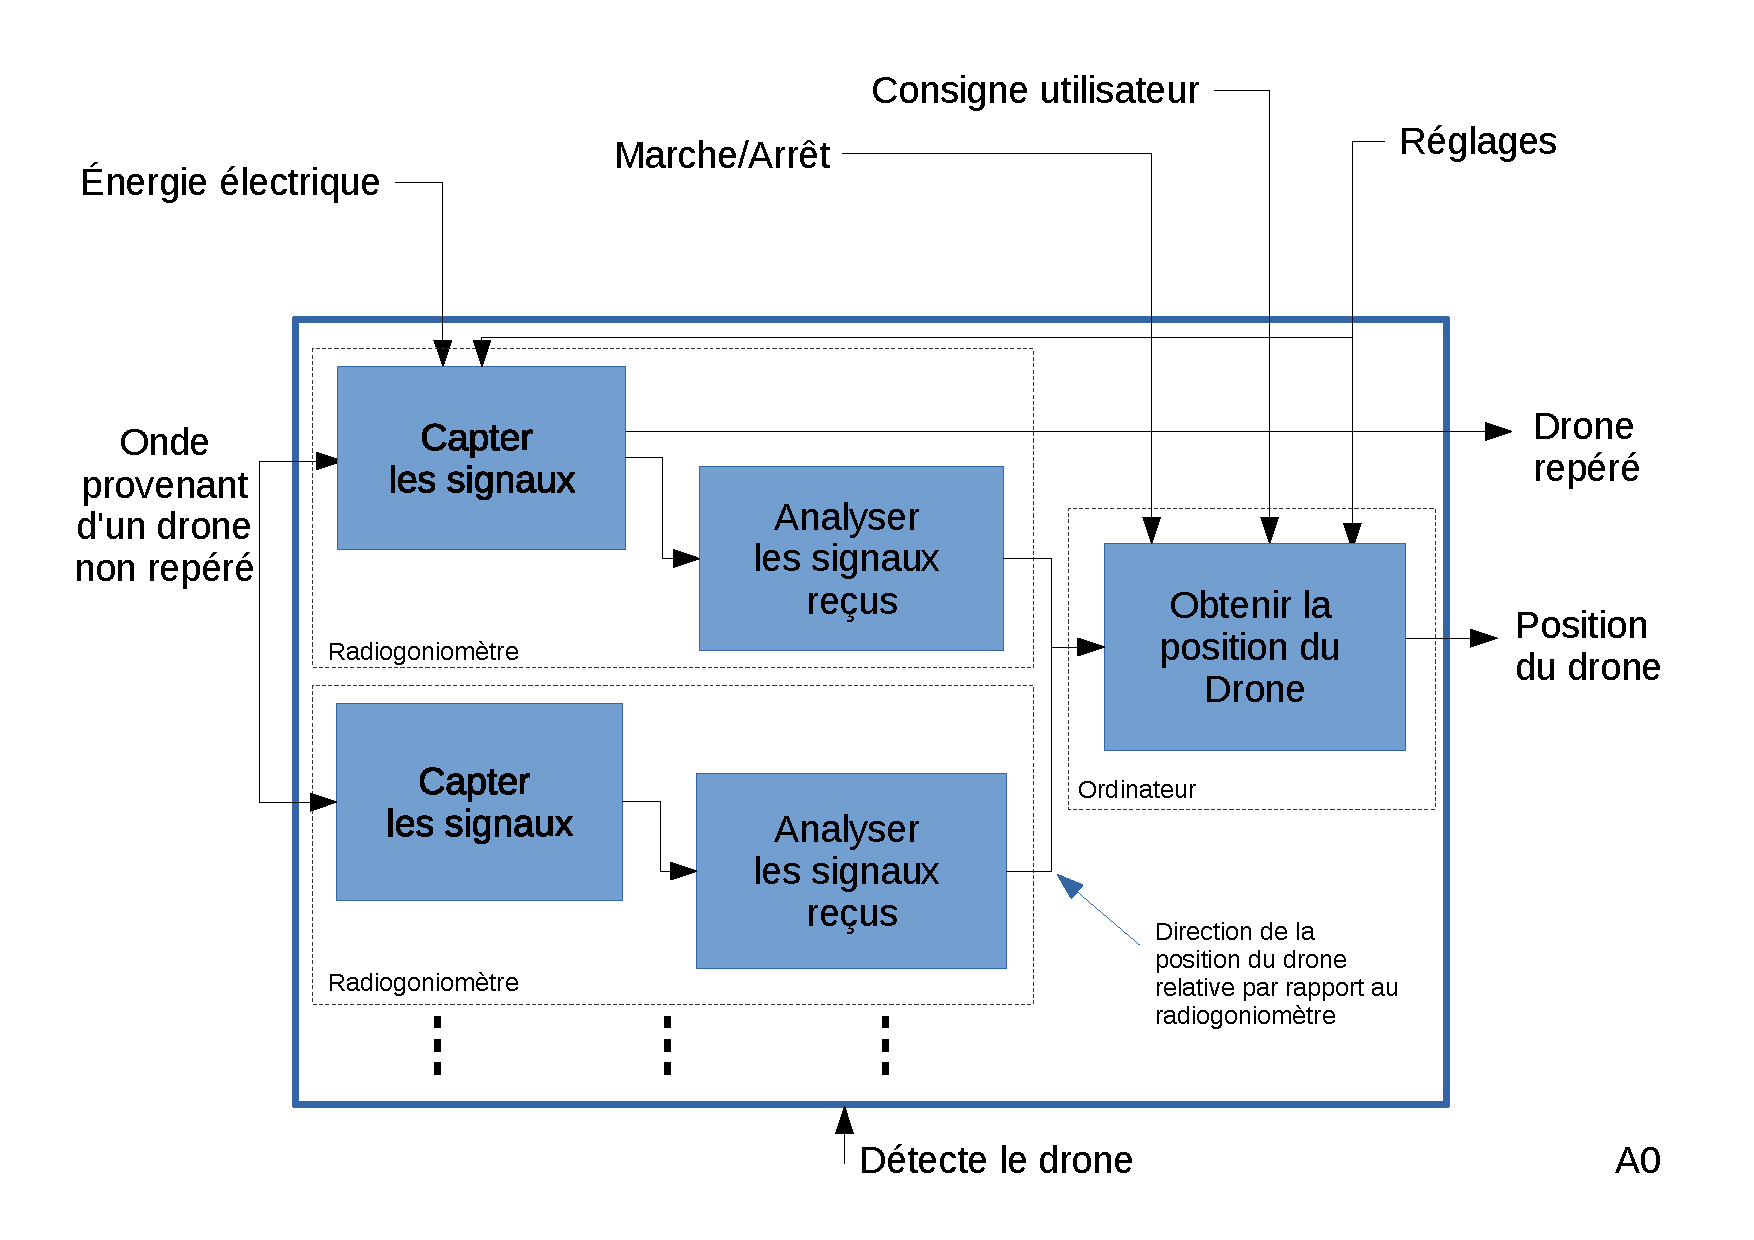
\includegraphics[width=\textwidth]{SADT_A0.pdf}
\captionof{figure}{SADT A0}

\parindent=15pt

Comme on peut le voir sur le SADT A0, nous avons découpé notre objectif en trois parties.

Dans un premier temps il faut capter les signaux. Pour cela il faut réaliser un balayage sur le radiogoniomètre pour détecter les bons signaux.

Ensuite, il faut analyser les signaux reçus pour s'assurer que nous sommes bien en présence d'un drone.

Enfin, il faut récupérer les données des radiogoniometres pour déterminer la position du drone.


\section{Listes des exigences fonctionnelles}

La liste des exigences fonctionnelles est située en Annexe dans le document TableauDesSpecification.xlsx

\section{Cahier des charges}

Le cahier des charges est situé en Annexe dans le document Cahier\_des\_charges.xlsx.




%%% Local Variables: 
%%% mode: latex
%%% TeX-master: "rapport_analyse"
%%% End: 